\newcommand{\chapter}[2][]{
	\newcommand{\chapname}{#2}
	\begin{flushleft}
		\begin{minipage}[t]{\linewidth}
			
\includegraphics[height=1cm]{hdht-logo.png}
			\hspace{0pt}	
			\sffamily\bfseries\large Bài  15.
			\begin{flushleft}
				\huge\bfseries #1
			\end{flushleft}
		\end{minipage}
	\end{flushleft}
	\vspace{1cm}
	\normalfont\normalsize
}
\chapter[Ba định luật Newton về chuyển động]{Ba định luật Newton về chuyển động}
\section{Lý thuyết}

\subsection{Định luật I Newton về chuyển động}
\subsubsection{Nội dung định luật}
Vật đang đứng yên sẽ tiếp tục đứng yên, đang chuyển động thẳng đều sẽ tiếp tục chuyển động thẳng đều, trừ khi có lực hoặc hợp lực khác không tác dụng lên vật. 
\subsubsection{Quán tính}
Quán tính là tính chất của mọi vật có xu hướng duy trì trạng thái chuyển động. 

Định luật I được gọi là định luật quán tính và chuyển động thẳng đều được gọi là chuyển động theo quán tính.

Hệ qui chiếu quán tính là hệ quy chiếu mà trong đó định luật 1 nghiệm đúng. 
\subsection{Định luật II Newton về chuyển động}
\subsubsection{Nội dung định luật}
Trong hệ quy chiếu quán tính, nếu một vật có khối lượng chịu tác dụng của lực, thì vật đó có gia tốc. Gia tốc này cùng hướng với lực tác dụng lên vật, có độ lớn tỉ lệ thuận với độ lớn của lực và tỉ lệ nghịch với khối lượng của vật.
\begin{equation*}
	\vec{a}=\dfrac{\vec F}{m},
\end{equation*}
trong đó:
\begin{itemize}
	\item $\vec F$ là lực tác dụng lên vật (N);
	\item m là khối lượng của vật (kg);
	\item $\vec a$ là gia tốc của vật ($\text{m/s}^2$).
\end{itemize}

\subsubsection{Khối lượng và quán tính}
Khối lượng là đại lượng đặc trưng cho mức quán tính của vật. Vật có mức quán tính lớn hơn thì khối lượng lớn hơn và ngược lại. 

%\subsubsection{Trọng lực - Trọng lượng}
%Trọng lực là lực của Trái Đất tác dụng vào vật gây ra cho chúng gia tốc rơi tự do. Trọng lực kí hiệu là $\vec P.$

%Ở gần Trái Đất, trọng lực có phương thẳng đứng, có chiều từ trên xuống và đặt vào một điểm đặc biệt của mỗi vật, gọi là trọng tâm của vật.


%Độ lớn của trọng lực tác dụng lên một vật gọi là trọng lượng của vật, kí hiệu là $P$. 

%Công thức tính trọng lực: 
%\begin{equation*}
%	\vec P=m\vec g.
%\end{equation*}

% Hung comment: mục này bỏ, vì khái niệm trọng lượng đã ghi là sai. Trọng lượng không phải độ lớn của trọng lực, vì như vậy thì không thể có ``hiện tượng không trọng lượng''. Trọng lượng là độ lớn của lực do vật tác dụng lên giá đỡ hoặc dây treo khi vật cân bằng trong trọng trường. Trường hợp vật được treo và cân bằng, vật có xu hướng kéo sợi dây làm dây căng, trọng lượng là độ lớn của lực căng dây. Trường hợp vật ở trên giá đỡ, vật có xu hướng ép lên giá đỡ, trọng lượng là độ lớn của lực nến này.

 
\subsection{Định luật III Newton về chuyển động}
\subsubsection{Nội dung định luật}
Trong mọi trường hợp, khi vật A tác dụng lên vật B một lực, thì vật B cũng tác dụng lại vật A một lực. Hai lực này có cùng giá, cùng độ lớn, nhưng ngược chiều.
\begin{equation*}
	{\vec F}_{\text{AB}}=-{\vec F}_{\text{BA}}.
\end{equation*}
\subsubsection{Lực và phản lực}
Một trong hai lực tương tác giữa hai vật gọi là lực tác dụng còn lực kia gọi là phản lực.

Lực và phản lực có những đặc điểm: 
\begin{itemize}
	\item Lực và phản lực luôn luôn xuất hiện (hoặc mất đi) đồng thời.
	\item Lực và phản lực có cùng giá, cùng độ lớn nhưng ngược chiều. Hai lực không phải là hai lực cân bằng, vì chúng đặt vào hai vật khác nhau.
\end{itemize}
\subsection{Chuyển động của vật và hệ vật}
Nếu các vật trong hệ liên kết với nhau bằng dây nối nhẹ không co giãn thì các vật trong hệ chuyển động với cùng một gia tốc
\begin{equation*}
	\vec a = \dfrac{\vec F_1 + \vec F_2 + ...}{m_1 + m_2+...}
\end{equation*}
\vspace{0.3cm}
\luuy{
\begin{itemize}
	\item Nếu trong hệ có một ròng rọc động, khi ròng rọc động đi được quãng đường $s$ thì vật treo ở đầu dây đi được quãng đường là $2s$. Vận tốc và gia tốc của vật cũng theo tỉ lệ đó.
	\item hệ gồm hai vật liên kết với nhau, khi có chuyển động tương đối giữa hai vật ta cần khảo sát từng vật riêng lẻ; còn khi hai vật  không có chuyển động tương đối với nhau  ta coi hai vật là một vật có khối lượng bằng tổng khối lượng của hai vật khi khảo sát.	
\end{itemize}
}
%Hung comment: ghi chú cũ về ròng rọc động là sai; ghi chú về hai vật chồng lên nhau là chưa tổng quát. 

\section{Mục tiêu bài học - Ví dụ minh họa}
\begin{dang}{Ghi nhớ định luật I Niu-tơn. \\ Nhận biết quán tính}
	\viduii{1}{Một chiếc xe buýt đang chạy trên đường thì tài xế phanh xe gấp. Một hành khách ngồi ở cuối xe phàn nàn rằng, do bác tài xế phanh xe gấp mà chiếc túi xách ở phía trước bay về phía anh ta làm anh ta bị đau. Người hành khách nói đúng hay sai? Em hãy giải thích?
	}
	{	\begin{center}
			\textbf{Hướng dẫn giải}
		\end{center}
		
		Người hành khách đã nói sai. Khi xe dừng lại đột ngột, túi xách theo quán tính phải bay về phía trước, không phải bay về phía sau.
		
	}
	\viduii{1}{\begin{enumerate}[label=\alph*.]
			\item Em hãy giải thích tại sao khi ta nhảy từ bậc cao xuống chân ta bị gập lại.  	
			\item Khi cán búa lỏng, tại sao ta có thể làm chặt lại bằng cách gõ mạnh đuôi cán xuống đất.
		\end{enumerate}
	}
	{	\begin{center}
			\textbf{Hướng dẫn giải}
		\end{center}
		
		\begin{enumerate}[label=\alph*.]
			\item Nhảy từ bậc cao xuống, chân chạm đất bị dừng lại ngay, nhưng người còn tiếp tục chuyển động theo quán tính nên làm chân gập lại.  	
			\item Khi gõ mạnh đuôi cán búa xuống đất, cán búa đột ngột dừng lại. Do quán tính đầu búa tiếp tục chuyển động gắn chặt vào cán búa. 
		\end{enumerate}
	}
\end{dang}	
\begin{dang}{Ghi nhớ định luật II Niu-tơn}
	\viduii{1}{Trong các cách viết công thức của định luật II Niu - tơn sau đây, cách viết nào đúng?
		\begin{mcq}(2)
			\item $\vec{F} = \dfrac{\vec{a}}{m}$.
			\item $\vec{a}=\dfrac{\vec{F}}{m}$. 
			\item $\vec{F} = - m\vec{a}$.
			\item $\vec{F} = ma.$
		\end{mcq}
% Hung comment: bản ghi cũ sai: đáp án B F=ma không phải định luật 2 Newton, mà chỉ là một hệ quả được suy ra bằng cách biên đổi toán học công thức của định luật II Newton.	
	}
	{	\begin{center}
			\textbf{Hướng dẫn giải}
		\end{center}
		
		Gia tốc của một vật cùng hướng với lực tác dụng lên vật. Độ lớn của gia tốc tỉ lệ thuận với độ lớn của lực và tỉ lệ nghịch với khối lượng của vật.
		\begin{equation}
			\vec{a}=\dfrac{\vec F}{m},
		\end{equation}
		
		\textbf{Đáp án: B}
	}
	\viduii{1}{Chọn câu phát biểu đúng?
		\begin{mcq}
			\item Nếu không có lực tác dụng vào vật thì vật không chuyển động được. 
			\item Lực tác dụng luôn cùng hướng với hướng biến dạng. 
			\item Vật luôn chuyển động theo hướng của lực tác dụng. 
%			\item Nếu có lực tác dụng lên vật thì vận tốc của vật bị thay đổi.
			\item Nếu vật chỉ chịu tác dụng của một lực khác không, thì vận tốc của vật sẽ bị thay đổi.
		\end{mcq}		
	}
	{	\begin{center}
			\textbf{Hướng dẫn giải}
		\end{center}
		
		Đáp án A: không có lực tác dụng thì vật vẫn có thể chuyển động thẳng đều nếu nó đang chuyển động thẳng đều. \\
		Đáp án B: Không có định luật nói về hướng của biến dạng dưới tác dụng của lực. \\
		Đáp án C: theo định luật II Newton, gia tốc luôn cùng hướng với lực tác dụng, chứ không phải vận tốc. \\
		Đáp án D: Nếu có lực tác dụng lên vật thì vật có gia tốc làm thay đổi vận tốc của vận. Đây là phát biểu đúng. 
		
		\textbf{Đáp án: D}
%	Hung comment: phát biểu cũ của đáp án D: ``nếu có lực tác dụng lên vật thì vận tốc của vật bị thay đổi'' là chưa đúng. Vẫn có trường hợp vật chịu tác dụng của nhiều lực, nhưng hợp lực bằng không thì vật vẫn không thay đổi vận tốc. 	
	}
\end{dang}
\begin{dang}{Ghi nhớ định luật III Niu-tơn, \\đặc điểm của cặp lực - phản lực}
	\viduii{1}{Trong một vụ tai nạn, một ô tô tải đâm vào một ô tô con đang chạy ngược chiều. Ô tô nào chịu lực lớn hơn? Hãy giải thích.
	}
	{	\begin{center}
			\textbf{Hướng dẫn giải}
		\end{center}
		
		Theo định luật III Niu-tơn , ô tô tải tác dụng vào ô tô con một lực thì ô tô con cũng tác dụng ngược lại ô tô tải một lực. Hai ô tô chịu lực bằng nhau về độ lớn, cùng phương nhưng ngược chiều nhau. Vì vậy, hai ô tô đều chịu một lực có độ lớn bằng nhau.
		
	}
	\viduii{1}{Khi đi bộ xa hoặc leo núi, ta chống gậy thì đỡ mỏi  chân. Tại sao?
		
	}
	{	\begin{center}
			\textbf{Hướng dẫn giải}
		\end{center}
		
		Khi đi bộ hoặc leo núi, chân ta phải đạp vào mặt đất, đất sẽ tác dụng một phản lực làm cho ta đi về phía trước. Động tác đó lặp đi lặp lại nhiều lần khiến cho cơ chân bị mỏi. Nếu chống gậy, bên cạnh việc đạp vào mặt đất, ta còn dùng tay ấn mạnh gậy đẩy mặt đất về phía sau, mặt đất sẽ tác dụng vào đầu gậy một phản lực hướng về phía trước. Phản lực này sẽ truyền qua gậy đến cơ thể làm cho ta dịch chuyển về phía trước. Như vậy chân không còn chịu toàn bộ tác dụng của mặt đất lên cơ thể nên chân đỡ mỏi hơn.
	}
\end{dang}

\begin{dang}{Áp dụng định luật III Niu-tơn}
	\viduii{3}{Một A vật có khối lượng $\SI{1}{kg}$ chuyển động với tốc độ $\SI{5}{m/s}$ va chạm vào một vật B đứng yên. Sau va chạm vật A chuyển động ngược trở lại với tốc độ $\SI{1}{m/s}$, còn vật B chuyển động với tốc độ $\SI{2}{m/s}$. Hỏi khối lượng của vật B bằng bao nhiêu?
	}
	{	\begin{center}
			\textbf{Hướng dẫn giải}
		\end{center}
		
		Chọn chiều dương là chiều chuyển động ban đầu của vật A và gọi $\Delta t$ là thời gian va chạm giữa hai vật, đinh luật III Niu-tơn cho ta
		\begin{align*}
			\vec{F}_{AB}&=-\vec{F}_{BA}\\
			\Rightarrow\quad m_A\vec{a}_A&=-m_B\vec{a}_B\\
			\Rightarrow\quad m_A\dfrac{\Delta \vec{v}_A}{\Delta t}&=-m_B\dfrac{\Delta\vec{v}_B}{\Delta t}\\	
			\Rightarrow\quad m_A(v_A-v_{A0})&=-m_B(v_B-v_{B0})\\
			\Rightarrow\quad \SI{1}{\kilogram}\cdot(\SI{-1}{\meter/\second}-\SI{5}{\meter/\second})&=-m_B(\SI{2}{\meter/\second}-\SI{0}{\meter/\second})		
		\end{align*}
		Phương trình trên cho nghiệm $m_B = \SI{3}{kg}.$
		
	}
	\viduii{3}{Một quả bóng, khối lượng $\SI{500}{g}$ bay với tốc độ $\SI{20}{m/s}$ đập vuông góc vào bức tường và bay ngược lại với tốc độ $\SI{20}{m/s}$. Thời gian va đập  là $\SI{0,02}{s}$. Lực do bóng tác dụng vào tường có độ lớn và hướng như thế nào?		
	}
	{	\begin{center}
			\textbf{Hướng dẫn giải}
		\end{center}
		
		Chọn chiều dương chuyển động là chiều bóng bay đập vào tường.
		
		Gia tốc mà quả bóng đạt được là
		
		$$a = \dfrac{v-v_0}{t}=\dfrac{-\SI{20}{\meter/\second}-\SI{20}{\meter/\second}}{\SI{0.02}{\second}} = -\SI{2000}{\meter/\second^2}.$$
		
		Lực do tường tác dụng vào bóng là
		
		$$F =ma =\SI{0.5}{\kilogram}\cdot(\SI{-2000}{\meter/\second})= -\SI{1000}{\newton}.$$
		Dấu trừ cho thấy lực do tường tác dụng vào bóng ngược với chiều chuyển động ban đầu của bóng. 
		
		Theo định luật III Niu-tơn, lực do bóng tác dụng vào tường có cùng độ lớn là \SI{1000}{\newton}, nhưng có chiều ngược lại, tức là cùng chiều chuyển động ban đầu của bóng.	
	}
	
\end{dang}
\begin{dang}{Biểu diễn hệ lực tác dụng lên hệ vật, \\áp dụng các định luật Niu-tơn \\để tính các đại lượng động lực học}

	\viduii{3}{Hai vật $m_1 = \SI{1}{kg}$, $m_2 = \SI{0,5}{kg}$ nối với nhau bằng sợi dây và được kéo lên thẳng đứng nhờ lực $F = \SI{18}{N}$ đặt lên vật I. Tìm gia tốc chuyển động và lực căng của dây. Coi dây là không giãn và có khối lượng không đáng kể.
		\begin{center}
			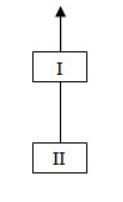
\includegraphics[scale=0.8]{../figs/VN10-PH-12-A-003-1-V2-01.jpg}
		\end{center}
	}
	{	\begin{center}
			\textbf{Hướng dẫn giải}
		\end{center}
		\begin{figure}[h]
			\centering
			\begin{subfigure}{0.5\linewidth}
				
			\end{subfigure}
		\end{figure}
		\begin{center}
			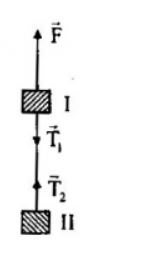
\includegraphics[scale=0.8]{../figs/VN10-PH-12-A-003-1-V2-02.jpg}
		\end{center}
		Các ngoại lực tác dụng lên hệ gồm trọng lực $\vec P_1$, trọng lực $ \vec P_2$, và lực $ \vec F$. 
		
		Phương trình định luật II Newton cho hệ có dạng 
			\begin{align}\label{IINewton-m1m2}
				m\vec{a}=\vec{F}+\vec{P}_1+\vec{P}_2.
			\end{align} 
		trong đó $m$ là khối lượng của hệ, bằng tổng khối lượng các vật trong hệ $m=m_1+m_2$. 
		
		Chọn chiều dương hướng lên. Gia tốc của hệ được suy ra khi chiếu phương trình định luật II Newton lên chiều dương 
		\begin{align*}
			ma&=F-P_1-P_2\\
			\Rightarrow\quad a&=\dfrac{F-P_1-P_2}{m_1+m_2}\\
				&=\dfrac{F-m_1g-m_2g}{m_1+m_2}\\
				&=\dfrac{\SI{18}{\newton}-\SI{1}{\kilogram}\cdot\SI{10}{\meter/\second^2}-\SI{0.5}{\kilogram}\cdot\SI{10}{\meter/\second^{2}}}{\SI{1}{\kilogram}+\SI{0.5}{\kilogram}}\\
				&=\SI{2}{\kilogram}		
		\end{align*}
			
		Xét riêng vật $m_2$, phương trình định luật II Newton cho vật này có dạng 
			\begin{align}\label{dlIINewton-m2}
				\vec{T}-\vec{P}_2&=m_2\vec{a}
			\end{align} 
		Chiếu phương trình này lên trục O$x$, ta tìm được độ lớn lực căng dây 
			\begin{align*}
				T-P_2&=m_2a\\
				\Rightarrow\quad T&=m_2a+P_2\\
				&=m_2(a+g)\\
				&=\SI{0.5}{\kilogram}\cdot(\SI{2}{\meter/\second^{2}}+\SI{10}{\meter/\second^{2}})\\
				&=\SI{6}{\newton}
			\end{align*}
		
		\luuy{
			\item Trong phương trình định luật II, ta chỉ xét các ngoại lực. Chẳng hạn, khi xét hệ gồm $m_1$ và $m_2$ (phương trình \ref{IINewton-m1m2}), ta không xét lực căng dây là lực tương tác giữa các thành phần bên trong hệ; trong khi đó ở phương trình \ref{dlIINewton-m2} khi xét riêng vật $m_2$ thì lực căng dây được xem là ngoại lực. 
			
		}
	}
	\viduii{3}{Một vật khối lượng $m$ treo vào trần một thang máy khối lượng $M$, $m$ cách sàn thang máy một khoảng $s$. Thang máy đang đi lên dưới tác dụng của một lực $F$ không đổi hướng lên.
		\begin{enumerate}[label=\alph*.]
			\item Tính gia tốc của $m$ và lực căng dây treo.
			\item Dây đứt đột ngột. Tính gia tốc của vật và buồng thang máy sau khi dây đứt và thời gian từ lúc đứt dây đến lúc vật $m$ chạm sàn.
		\end{enumerate}
		
	}
	{	\begin{center}
			\textbf{Hướng dẫn giải}
		\end{center}
		
		\begin{center}
			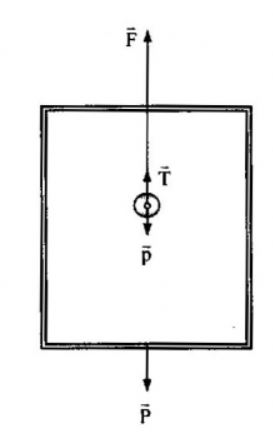
\includegraphics[scale=0.5]{../figs/VN10-PH-12-A-003-1-V2-03.jpg}
		\end{center}
		
		\begin{enumerate}[label=\alph*.]
			\item Gia tốc của $m$ và lực căng của dây treo
			
			- Chọn chiều dương hướng lên.
			
			- Các ngoại lực tác dụng lên hệ ``thang máy và người'' là: lực $\vec F$, các trọng lực $\vec P$, $\vec p$. Theo định luật II Newton:
				\begin{align*}
					\vec F + \vec P + \vec  p &= (M+m)\vec a\\
					\Rightarrow\quad a &=\dfrac{F - (M+m)g}{M+m}.
				\end{align*}

			
			- Xét riêng vật $m$
			\begin{align*}
				T - p &=ma \\
				\Rightarrow\quad T &= m(g+a) \\
				\Rightarrow\quad T &= \dfrac{mF}{M+m}.
			\end{align*}
			
			\item Giả sử khi dây đứt, hệ gồm thang máy và vật đang đi lên với vận tốc $v_0$. Ta chọn gốc thời gian là lúc thang máy đứt, hệ trục hướng lên, gốc tọa độ là vị trí sàn thang máy khi đó. 
			
			Khi dây treo vật đứt, vật $m$ chỉ còn chịu tác dụng của trọng lực nên có gia tốc là $\vec{g}$ hướng xuống. 
			
			Thang máy khi đó chịu tác dụng của hai lực là $\vec{F}$ hướng lên và trọng lực hướng xuống nên có gia tốc 
				\begin{align*}
					a=\dfrac{F-P}{M}=\dfrac{F}{M}-g
				\end{align*}		
			
			Phương trình chuyển động của vật và của sàn thang máy là 
				\begin{align*}
					x_m&=s+v_0t-\dfrac{1}{2}gt^2,
					x_M&=v_0t+\dfrac{1}{2}at^{2}.
				\end{align*}
			Khi vật chạm sàn
				\begin{align*}
					x_m&=x_M\\
					\Rightarrow\quad s+v_0t-\dfrac{1}{2}gt^2&=v_0t+\dfrac{1}{2}at^{2}\\
					\Rightarrow\quad t&=\sqrt{\dfrac{2s}{a+g}}\\
					&=\sqrt{\dfrac{2sM}{F}}
				\end{align*}
			
%			Gia tốc của vật và buồng thang máy sau khi đứt dây và thời gian từ lúc dây đứt đến lúc $m$ chạm sàn.
			
%			- Khi đứt dây: $F =0 \Rightarrow a_2 =-g$: vật $m$ không gắn với thang máy nữa nên $a_1 = \dfrac{F}{M} - g.$
			
%			- Thời gian từ lúc dây đứt đến lúc chạm sàn:
			
%			+ Chọn hệ quy chiếu gắn với thang máy. 
			
%			$$a' =a_1 +g = \dfrac{F}{M}$$.
			
%			+ Thời gian rơi của $m$ khi dây đứt là:
			
%			$$ t=\sqrt {\dfrac{2s}{a'}} = \sqrt{\dfrac{2sM}{F}}.$$
		
%Hưng comment: không nên sử dụng hệ qui chiếu gắn với thang máy vì: 1) chương trình không có bài nào về hệ qui chiếu phi quán tính. 2) trong chương trình chỉ có công thức cộng vận tốc, không có công thức cộng gia tốc.			
			
		\end{enumerate}	
	}
	
	\viduii{3}{Cho hệ vật như hình vẽ có $m_1 = 2m_2$. Lực căng của dây treo ròng rọc là $\SI{52,3}{N}$. Tìm gia tốc chuyển động của mỗi vật, lực căng của dây treo vật. Lấy $g = \SI{9,8}{m/s^2}$.
		
		\begin{center}
			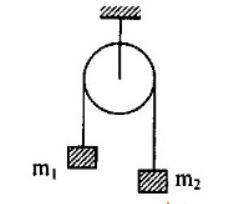
\includegraphics[scale=0.5]{../figs/VN10-PH-12-A-003-1-V2-04.jpg}
		\end{center}
	}
	{	\begin{center}
			\textbf{Hướng dẫn giải}
		\end{center}
		
		Các lực tác dụng lên ròng rọc được biểu diễn trên hình vẽ.
		\begin{center}
			\begin{tikzpicture}[>=Latex]
				\draw[thick] (0,0) circle (5mm);
				\draw[thick,->](-0.5,0)--++(0,-1)node[below]{$T$};
				\draw[thick,->](0.5,0)--++(0,-1)node[below]{$T$};
				\draw[thick,->](0,0)--++(0,1)node[above]{$T'$};
			\end{tikzpicture}
		\end{center}
		
		Vì ròng rọc được cố định nên các lực tác dụng lên ròng rọc triệt tiêu nhau, do đó		
		$$ T' = 2T \Rightarrow T = \dfrac{T'}{2} = \SI{26,15}{N}.$$
		
		Đối với hệ vật, $m_1 > m_2$ nên $m_1$ đi xuống, $m_2$ đi lên. Chiều dương được chọn là chiều chuyển động của hệ.
		
		\begin{center}
			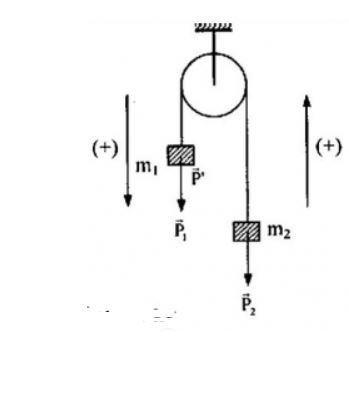
\includegraphics[scale=0.6]{../figs/VN10-PH-12-A-003-1-V2-05.jpg}
		\end{center}	
		Áp dụng định luật II Newton:
			\begin{align*}
				\vec P_1 + \vec P_2 =(m_1 + m_2) \vec a.
			\end{align*}
		Chiếu biểu thức trên lên chiều dương đã chọn:
			\begin{align*}
				P_1 - P_2 &=(m_1+m_2)a \\
				\Rightarrow\quad a &= \dfrac{m_1 - m_2}{m_1 +m_2} g\\
				&= \dfrac{2m_2 -m_2}{2m_2 + m_2}g	\\
				&= \SI{3,27}{m/s^2}.
			\end{align*}
	
		Xét riêng vật $m_2$ 
		
		$$T - P_2 =m_2a \Rightarrow T -m_2g = m_2a \Rightarrow m_2 = \dfrac{T}{g+a} = \SI{2}{kg}.$$
		
		Suy ra $m_1 =2m_2 = \SI{4}{kg}.$
	}
	
\end{dang}